
This section is devoted to fully describe our novel proposal called \textit{Variable Space Diversity based MOEA} 
(\VSDMOEA{})~\footnote{The source code in C++ is freely available in \url{https://github.com/joelchaconcastillo/VSD-MOEA.git}}.
%
The novelty of \VSDMOEA{} appears in the replacement phase, which incorporates
the use of variable space diversity and a novel objective space density estimator. 
%
The main principle behind the design of the novel replacement is to use the stopping criterion and 
elapsed generations with the aim of gradually moving from exploration to exploitation during the search process.
%
Note that this principle might be incorporated in any of the three categories of \MOEAS{}.
%
In this paper, our decision was to incorporate it in a dominance-based approach.
%
Note that this category has been particularly suitable for problems with two and three objectives.
%
Thus, some of our design decisions might not be convenient for dealing with many-objective optimization problems.

The general framework of \VSDMOEA{} is quite standard.
%
Algorithm~\ref{alg:vsd-moea} shows the pseudo-code of \VSDMOEA{}.
%
The parent selection is performed with binary tournament based on the dominance raking with ties broken randomly.
%
The variation stage is based on applying the well-known Simulated Binary Crossover (SBX) 
and polynomial mutation~\cite{Joel:SBX1994, Joel:Mutation}.
%
Thus, the contribution appears in the replacement phase.
%
The rest of this section is devoted to describe the replacement phase, including the novel objective space density 
estimator.

\begin{algorithm}[t]
\algsetup{linenosize=\tiny}
	\caption{Main procedure of VSD-MOEA} 
	\begin{small}
\begin{algorithmic}[1]
 	\STATE \textbf{Initialization}: Generate an initial population $P_0$ with $N$ individuals.
	\STATE \textbf{Evaluation}: Evaluate all individuals in the population.
	\STATE Assign $t=0$
	\WHILE{ (not stopping criterion)  }
	   \STATE \textbf{Mating selection}: Fill the mating pool by performing binary tournament selection on $P_t$, 
		 based on the non-dominated ranks (ties are broken randomly).
	   \STATE \textbf{Variation}: Apply SBX crossover and Polynomial mutation to the mating pool to create a child population $Q_t$.
		 \STATE \textbf{Evaluation}: Evaluate all individuals in $Q_t$.
	   \STATE \textbf{Survivor selection}: Generate $P_{t+1}$ by applying the replacement scheme 
		 described in Algorithm \ref{alg:Replacement_Phase}, using $P_t$ and $Q_t$ as input.
	   \STATE $t=t+1$
	\ENDWHILE
	\end{algorithmic}
	\end{small}
\label{alg:vsd-moea}
\end{algorithm}


\subsection{Replacement Phase of VSD-MOEA}

The replacement phase of \EAS{} is in charge of deciding in each generation which are the survivors 
among the members of the previous population and offspring.
%
The novel replacement promotes a gradual movement from exploration to exploitation, which has been a quite 
beneficial principle in the design of single-objective optimizers~\cite{Joel:MULTI_DYNAMIC}.
%
Particularly, the replacement phase operates as follows.
%
First, the members of the previous population and offspring are joined in a multi-set with $2 \times N$ individuals.
%
%Then, for each objective a high-quality candidate solution is selected to survive.
%
%The specific process to perform this selection is detailed later.
%
Then, an iterative process that selects an additional
individual at each iteration is used to pick up the $N$ survivors. 
%
In order to take into account the diversity in the decision space, the Distance to Closest Survivor (\DCS{}) of each
individual is calculated at each iteration.
%
Thus, the \DCS{} of an individual $I$ is calculated as $\displaystyle{\min_{s \in S}\ Distance(I, s)}$,
where $S$ is the multi-set containing the currently selected survivors. 
%
Normalized Euclidean distances are considered, so in order to calculate distances between any two individual $A$ and $B$, 
Eq. (\ref{eqn:distance}) is applied.
%
In the first iteration, the $S$ multi-set is empty, so the \DCS{} of each individual is infinity.
%
\begin{equation}\label{eqn:distance}
Distance(A, B) =   \left ( \frac{1}{n}  \sum_{i=1}^n \left ( \frac{A_i - B_i}{x_i^{(U)} - x_i^{(L)}} \right )^2  \right)^{1/2}
\end{equation}

Note that individuals with larger \DCS{} values are those that contribute more significantly to promote exploration.
%
In order to avoid an excessive decrease of the exploration degree, individuals with a \DCS{} value lower 
than a threshold value are penalized.
%
Then, among the non-penalized individuals, an objective space density estimator is used to select the additional
survivor of the iteration.
%
In our case, the novel density estimator described in the next subsection is used. 
%
Note that it might happen that all individuals are penalized.
%
In such a case, the individual with the largest \DCS{} is selected.

\begin{figure}[t]
\centering
%



\tikzset{every picture/.style={line width=0.75pt}} %set default line width to 0.75pt        

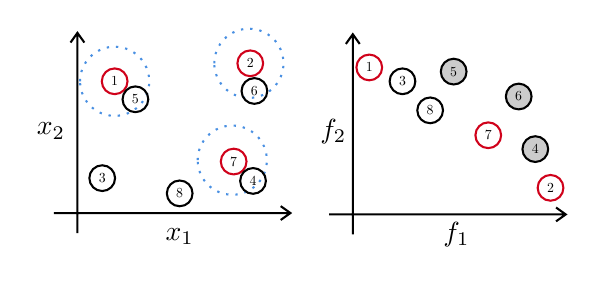
\begin{tikzpicture}[x=0.5pt,y=0.5pt,yscale=-1,xscale=1]
%uncomment if require: \path (0,300); %set diagram left start at 0, and has height of 300

%Shape: Circle [id:dp5136866411017809] 
\draw  [color={rgb, 255:red, 74; green, 144; blue, 226 }  ,draw opacity=1 ][dash pattern={on 0.84pt off 2.51pt}] (69,105) .. controls (69,91.19) and (80.19,80) .. (94,80) .. controls (107.81,80) and (119,91.19) .. (119,105) .. controls (119,118.81) and (107.81,130) .. (94,130) .. controls (80.19,130) and (69,118.81) .. (69,105) -- cycle ;
%Shape: Circle [id:dp3061612047883613] 
\draw  [color={rgb, 255:red, 74; green, 144; blue, 226 }  ,draw opacity=1 ][dash pattern={on 0.84pt off 2.51pt}] (166,92) .. controls (166,78.19) and (177.19,67) .. (191,67) .. controls (204.81,67) and (216,78.19) .. (216,92) .. controls (216,105.81) and (204.81,117) .. (191,117) .. controls (177.19,117) and (166,105.81) .. (166,92) -- cycle ;
%Shape: Axis 2D [id:dp3645341276574614] 
\draw  (50,200.22) -- (221,200.22)(67.1,70) -- (67.1,214.69) (214,195.22) -- (221,200.22) -- (214,205.22) (62.1,77) -- (67.1,70) -- (72.1,77)  ;
%Shape: Circle [id:dp595877391054507] 
\draw  [color={rgb, 255:red, 74; green, 144; blue, 226 }  ,draw opacity=1 ][dash pattern={on 0.84pt off 2.51pt}] (154,162) .. controls (154,148.19) and (165.19,137) .. (179,137) .. controls (192.81,137) and (204,148.19) .. (204,162) .. controls (204,175.81) and (192.81,187) .. (179,187) .. controls (165.19,187) and (154,175.81) .. (154,162) -- cycle ;
%Shape: Axis 2D [id:dp14963900792703488] 
\draw  (249,201.22) -- (420,201.22)(266.1,71) -- (266.1,215.69) (413,196.22) -- (420,201.22) -- (413,206.22) (261.1,78) -- (266.1,71) -- (271.1,78)  ;

% Text Node
\draw  [color={rgb, 255:red, 208; green, 2; blue, 27 }  ,draw opacity=1 ]  (94, 105) circle [x radius= 9.3, y radius= 9.3]   ;
\draw (94,105) node [scale=0.5] [align=left] {1};
% Text Node
\draw  [color={rgb, 255:red, 0; green, 0; blue, 0 }  ,draw opacity=1 ]  (109, 118) circle [x radius= 9.3, y radius= 9.3]   ;
\draw (109,118) node [scale=0.5] [align=left] {5};
% Text Node
\draw  [color={rgb, 255:red, 208; green, 2; blue, 27 }  ,draw opacity=1 ]  (192, 92) circle [x radius= 9.3, y radius= 9.3]   ;
\draw (192,92) node [scale=0.5] [align=left] {2};
% Text Node
\draw    (195, 112) circle [x radius= 9.3, y radius= 9.3]   ;
\draw (195,112) node [scale=0.5] [align=left] {6};
% Text Node
\draw  [color={rgb, 255:red, 208; green, 2; blue, 27 }  ,draw opacity=1 ]  (180, 163) circle [x radius= 9.3, y radius= 9.3]   ;
\draw (180,163) node [scale=0.5] [align=left] {7};
% Text Node
\draw    (194, 177) circle [x radius= 9.3, y radius= 9.3]   ;
\draw (194,177) node [scale=0.5] [align=left] {4};
% Text Node
\draw    (141, 186) circle [x radius= 9.3, y radius= 9.3]   ;
\draw (141,186) node [scale=0.5] [align=left] {8};
% Text Node
\draw    (85, 175) circle [x radius= 9.3, y radius= 9.3]   ;
\draw (85,175) node [scale=0.5] [align=left] {3};
% Text Node
\draw  [color={rgb, 255:red, 208; green, 2; blue, 27 }  ,draw opacity=1 ]  (278, 95) circle [x radius= 9.3, y radius= 9.3]   ;
\draw (278,95) node [scale=0.5] [align=left] {1};
% Text Node
\draw  [color={rgb, 255:red, 0; green, 0; blue, 0 }  ,draw opacity=1 ][fill={rgb, 255:red, 0; green, 0; blue, 0 }  ,fill opacity=0.2 ]  (339, 98) circle [x radius= 9.3, y radius= 9.3]   ;
\draw (339,98) node [scale=0.5] [align=left] {5};
% Text Node
\draw  [color={rgb, 255:red, 208; green, 2; blue, 27 }  ,draw opacity=1 ]  (409, 182) circle [x radius= 9.3, y radius= 9.3]   ;
\draw (409,182) node [scale=0.5] [align=left] {2};
% Text Node
\draw  [fill={rgb, 255:red, 0; green, 0; blue, 0 }  ,fill opacity=0.2 ]  (386, 116) circle [x radius= 9.3, y radius= 9.3]   ;
\draw (386,116) node [scale=0.5] [align=left] {6};
% Text Node
\draw  [color={rgb, 255:red, 208; green, 2; blue, 27 }  ,draw opacity=1 ]  (364, 144) circle [x radius= 9.3, y radius= 9.3]   ;
\draw (364,144) node [scale=0.5] [align=left] {7};
% Text Node
\draw  [fill={rgb, 255:red, 0; green, 0; blue, 0 }  ,fill opacity=0.2 ]  (398, 154) circle [x radius= 9.3, y radius= 9.3]   ;
\draw (398,154) node [scale=0.5] [align=left] {4};
% Text Node
\draw    (322, 126) circle [x radius= 9.3, y radius= 9.3]   ;
\draw (322,126) node [scale=0.5] [align=left] {8};
% Text Node
\draw    (302, 105) circle [x radius= 9.3, y radius= 9.3]   ;
\draw (302,105) node [scale=0.5] [align=left] {3};
% Text Node
\draw (141,217) node   {$x_{1}$};
% Text Node
\draw (48,141) node   {$x_{2}$};
% Text Node
\draw (341,216) node   {$f_{1}$};
% Text Node
\draw (252,141) node   {$f_{2}$};


\end{tikzpicture}


%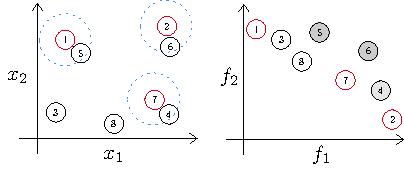
\includepdf[pages=-]{Images/Diagram.pdf}
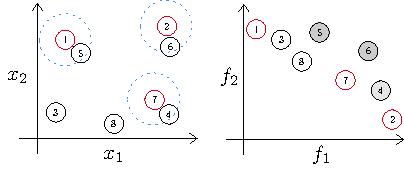
\includegraphics[width=0.45\textwidth]{Images/Diagram.pdf}
\caption{Penalty Method of the Replacement Phase - The left side represents the variables space and the right side the 
objective space.} \label{fig:Hypersphere}
\end{figure}



In order to better understand the penalty method, it can be visualized in the following way.
%
After selecting each survivor, a hyper-sphere 
centered in such a candidate solution --- in the variable space --- is created.
%
Then, all the individuals that are inside a hyper-sphere are penalized and the objective space estimator takes 
into account only the survivors and non-penalized individuals.
%
This is illustrated in Fig.~\ref{fig:Hypersphere}, which represents a state where three individuals have been 
selected to survive and an additional survivor must be picked up.
%
The left side shows individuals in the variable space.
%
Current survivors are marked with a red border and each one of them is surrounded by a blue dash circle with 
radius $D_t$.
%
In this situation, the penalized individuals are the number 4, 5, and 6.
%
In the objective space --- right side --- penalized individuals are shown with gray background, indicating
that the objective space density estimator does not take them into account.

Since using a large radius for the hyper-spheres induces a large degree of 
exploration, it makes sense to reduce this value during the optimization process.
%
This is precisely one of the keys of our proposal.
%
The sizes of the hyper-spheres are modified dynamically by taking into account the stopping 
criterion and elapsed generations.
%
Particularly, the radius is decreased in a linear way starting from an initial distance.
%
This means that in the initial phases exploration is promoted.
%
However, as the size of the radius decreases only very close individuals are penalized, meaning that more 
exploitation is allowed.
%
Note that this method requires a parameter which is the initial radius of the 
hyper-spheres or initial threshold value.
%
This parameter is denoted as $D_I$. 
%
Setting this parameter with a large value might provoke the penalization of a lot of individuals,
thus non-useful diversity might be maintained.
%
However, too small values might not prevent fast convergence and therefore the approach  
might behave as a traditional non-diversity based \MOEA{}.
%
The robustness of the proposal with respect to this additional parameter is studied in our experimental validation.

Algorithm~\ref{alg:Replacement_Phase} fully describes the replacement phase of \VSDMOEA{}.
%
First, the population of the previous generation ($P_t$) and the offspring ($Q_t$) are joined
in $R_t$ (line \ref{alg:1}).
%
The multi-set $R_t$ contains, at each iteration, the remaining non-penalized individuals that might be selected 
to survive.
%
The population of survivors ($P_{t+1}$) and the set containing the penalized individuals are initialized to
the empty set (lines \ref{alg:2} and \ref{alg:3}).
%
Then, the threshold value ($D_t$) that is used to penalize too close individuals is calculated (line \ref{alg:4}).
%
Note that $D_I$ denotes the initial threshold value, $G_{Elapsed}$ is the amount of generations that have 
been evolved, and $G_{End}$ is the stopping criterion, i.e. the number of generations that are to be evolved 
in the execution of \VSDMOEA{}.
%
The linear decrease is calculated so that after the $50\%$ of the generations, the $D_t$ value is lower than 0, 
meaning that no penalties are performed.
%
This means that in the first $50\%$ of the generations, more exploration than in traditional MOEAs is induced.
%

\begin{algorithm}[t]
\algsetup{linenosize=\tiny}
	\caption{Replacement Phase of VSD-MOEA} 
\begin{small}
\begin{algorithmic}[1]
\STATE Input: $P_t$ (Population of current generation), $Q_t$ (Offspring of current Generation)
    	\STATE Output: $P_{t+1}$ 
        \STATE $R_t = P_t \cup Q_t$ \label{alg:1}
        \STATE $P_{t+1} = \emptyset$ \label{alg:2}
        \STATE $Penalized = \emptyset$ \label{alg:3}
				\STATE $D_t = D_I - D_I * \frac{G_{Elapsed}}{0.5*G_{End}}$ \label{alg:4}
%				\FOR{$k \in {1...M}$}\label{alg:5}
%					\STATE Move to $P_{t+1}$ the individual that optimize $AF_k$ (Eq.~\ref{eqn:extremes}) \label{alg:5b}
%				\ENDFOR
        \WHILE{ $|P_{t+1}|$ $\leq$ N } \label{alg:6}
					\STATE Compute $DCS$ of individuals in $R_t$ with $P_{t+1}$ used as reference set \label{alg:7}
					\STATE Move to $Penalized$ the individuals in $R_t$ with $DCS < D_t$  \label{alg:8}
        	\IF{$R_t$ is empty} \label{alg:9}
						\STATE Compute $DCS$ of individuals in $Penalized$ with $P_{t+1}$ used as reference set \label{alg:10}
						\STATE Move to $R_t$ the individual in $Penalized$ with largest $DCS$ \label{alg:11}
        	\ENDIF
					\STATE Identify the first front ($F$) in $R_t \cup P_{t+1}$ with an individual $I \in R_t$ \label{alg:12}
					\STATE Use the novel density estimator (Algorithm~\ref{alg:Density_Estimator}) to select a new survivor 
					from $F$ and move it to $P_{t+1}$\label{alg:13}
        \ENDWHILE
    	\RETURN $P_{t+1}$ \label{alg:14}
	\end{algorithmic}
\end{small}
\label{alg:Replacement_Phase}
\end{algorithm}

Then, an iterative process that selects an individual at each iteration is executed until the survivors
set contains $N$ individuals (line \ref{alg:6}).
%
The iterative process works as follows.
%
First, the \DCS{} value of each remaining non-penalized individual is calculated (line \ref{alg:7}).
%
Then, those individuals with a \DCS{} value lower than $D_t$ are moved to the set of penalized individuals (line \ref{alg:8}).
%
If all the remaining individuals are penalized (line \ref{alg:9}), it means that the amount of exploration is lower than the
desired one.
%
Thus, the individual with the largest \DCS{} value is recovered, i.e. moved to the non-penalized individuals 
set (lines \ref{alg:10} and \ref{alg:11}) and consequently it survives.
%
Finally, the objective space is taken into account.
%
Specifically, candidate non-penalized individuals and current survivors are joined.
%
Then, the well-known non-dominated sorting procedure~\cite{Joel:NSGAII} is executed with such a set, stopping as soon as a front with 
a candidate individual is found, i.e. with an individual of $R_t$ (line \ref{alg:12}).
%
Then, taking the identified front as input, a novel objective space density estimator is used to select
the next survivor (line \ref{alg:13}).
%
The specific way in which the contribution to diversity in the objective space of each individual is measured is described in the next section.
%

%Note also that, as part of the diversity calculation of the variable space, a metric should be selected.
%
%Since our experimental validation is performed with a continuous domain, the normalized Euclidean distance is used.
%%
%However, in discrete domains other distance metrics such as the Manhattan, or the Hamming distance might be considered, and the definition of
%such distance might affect the performance of the approach~\cite{Segura:17}.


%The main idea of replacement phase dwell in compute the contribution by each individual to diversity  in both spaces.
%
%Hence in each iteration just one individual is selected as survivor until the size of population is reached.
%
%Consequently this methodology separate the suitable candidates based in diversity of the variable space, afterward the best candidate in objective space is selected.
%

%
%The figure \ref{fig:Hypersphere} shows one iteration of the Replacement Phase where the reference individuals are $\{1, 2, 7\}$ and candidate individuals are $\{3, 4, 5, 6, 8\}$. 
%
%The individuals $\{4, 5, 6\}$ are moved to penalized set, since that each one is inside of a hypersphere (gray dotted circles) related to a reference individual.
%
%Finally, the candidate solutions are $\{2, 8\}$, due that both belongs to the same rank, the solution $8$ is selected since it has a better contribution to the diversity in the objective space.

%
%
%
%
% %The function definitions from algorithm~\ref{alg:Replacement_Phase} are explained as follow:
% %
% \begin{itemize}
% \item Diversity\_Variable\_Space(A,B): for each individual from set A an euclidean distance is computed in variable space to the closest solution from the set B.
% \item Diversity\_Objective\_Space(A,B): for each individual from set A an euclidean distance is computed in objective space to the closest solution from the set B.
%\end{itemize}
%
%
%

%ESto hay que moverlo a Experimental Validation
%Due that the initial diversity is influenced by  $D_I$ parameter, several experiments with different values have been realized.
%
%Accordingly that each dimension is normalized in the unity, the maximal hypersphere of the variable decisions is denoted by $\sqrt{N}$ where $N$ is the dimension of the variable space. 
%
%Under those circumstances, the hypersphere with radius $\sqrt{N}$ will cover outside from the bounds, for this reason it is multiplied by a factor $k$  resulting in the formula$D_I = k * \sqrt[]{N}  \rightarrow k \in (0,1)$.
%
%Empirically, the ideal configuration that provides quality solutions is $k=0.25$ .
%
%Additionally, the algorithm empirically is enough stable, given that different values of $k$ does not provide drastically differences in the solutions.

\subsection{A Novel Density Estimator for the Objective Space}
\label{subsection:density}

\begin{algorithm}[t]
\algsetup{linenosize=\tiny}
	\caption{Density estimator} 
\begin{small}
\begin{algorithmic}[1]
\STATE Input: $P_{t+1}$ (Survivors), $R_t$ (Candidates), $F$ (Current front)
    	\STATE Output: $I \in R_t$ 
	\STATE $FP = P_{t+1} \cap F$ \label{alg:FP}
	\STATE $FR = R_{t} \cap F$ \label{alg:FR}
        \FOR{$k \in$ number of objectives}\label{alg:density_for}
	      \STATE Select the best individual $I \in F$ of $k$ according to Eq.~\ref{eqn:extremes}.\label{alg:density_1}
	  	\IF{ $I \in FR$}
	  	 \RETURN $I$ \label{alg:density_2}
	  	\ENDIF
	\ENDFOR\label{alg:density_endfor}
	\STATE $MaxID = 0$ \label{alg:density_for2}
	\FOR{ $ Ic \in FR$}
	\STATE $Improvement = \displaystyle{\min_{s \in FP}\ ID(Ic, s)}$ 
	\IF{ $Improvement > MaxID$} \label{alg:density_if2}
	   \STATE $MaxID = Improvement$
	   \STATE $I = Ic$ 
	\ENDIF \label{alg:density_endif2}
	\ENDFOR	\label{alg:density_endfor2}
    	\RETURN $I$ \label{alg:density_4}
	\end{algorithmic}
\end{small}
\label{alg:Density_Estimator}
\end{algorithm}

Since the dominance definition is not related to the preservation of diversity in the objective space,
dominance-based \MOEAS{} usually incorporate objective-space density estimators to promote the survival
of diverse individuals.
%
As it was previously described, our density estimator selects a new survivor from the front identified
in line \ref{alg:13} of Algorithm~\ref{alg:Replacement_Phase}.
%
This front (referred in Algorithm~\ref{alg:Density_Estimator}  as $F$) contains at least one individual belonging to $R_t$ and it might also contain some elements 
of $P_{t+1}$.
%
The aim behind the selection of the next survivor is to pick up an individual of the input front
that contributes significantly in terms of objective-space quality and diversity. % to $R_t$.

Algorithm~\ref{alg:Density_Estimator} describes the selection of the next survivor.
%
First, the sets $FP$ and $FR$ are identified (lines \ref{alg:FP} and \ref{alg:FR}).
%
$FP$ contains the current survivors that are in $F$, whereas $FR$ contains
the remaining candidate individuals that are in $F$.
%
Then, similarly to most state-of-the-art algorithms, an action to promote the selection of boundary solutions
is included.
%
Note that selecting the best solution for each objective might provoke some drawbacks related to accepting an small improvement
in an objective at the cost of important worsening in other objectives~\cite{deb2016optimality}.
%
To solve this issue augmented functions can be applied, which has been the alternative used in this paper.
%
Particularly, iteratively, for each objective $k$ the candidate solution that minimizes the Augmented Function (AF)
given in Eq.~\ref{eqn:extremes} is identified (lines \ref{alg:density_for} to \ref{alg:density_endfor}).
%
If such an individual belongs to $FR$, i.e., it has not been selected yet as a survivor, the next survivor is such an individual
and the process finalizes (line \ref{alg:density_2}).
%
Note that, augmented functions usually take into account weight vectors with the aim of dealing with objectives
that present very different scales.
%
Since benchmarks that have similar scales in each objective have been used in this paper, there was no need to apply
such weight vectors.

\begin{equation}\label{eqn:extremes}
AF_k (\vec{x}) = f_k(\vec{x}) + 10^{-4} \times  \sum_{j=1}^M f_j( \vec{x} )
\end{equation}

In cases where the individuals that optimize each $AF_K$ function are already in $P_{t+1}$, a contribution
to objective-space diversity is calculated for each individual in $FR$ (lines \ref{alg:density_for2} to \ref{alg:density_4}).
%
This contribution is calculated by taking into account the current survivors of the front ($FP$).
%
%Then, the one with a higher contribution is selected (line XXX).
%
Particularly, the ``Improvement Distance'' ($ID$) defined for the indicator IGD+~\cite{Joel:Inverted_Generational_Distance_Plus}
is used.
%
The $ID$ of an individual $A$ with respect to an individual $B$ is calculated by taking into account only the objectives
where $A$ is better.
%
Specifically, Eq. (\ref{eq:ImprovementDistance}) is used.

\begin{equation} \label{eq:ImprovementDistance}
\begin{split}
 ID(A, B) = &  \left (\sum_{i=1}^M \left (max(0, B_i - A_i \right ))^2  \right)^{1/2}
\end{split}
\end{equation}

Thus, the contribution of each member of $FP$ is calculated as $\displaystyle{\min_{s \in FP}\ ID(I, s)}$.
%
Then, the individual with the highest contribution is selected as the next survivor (lines \ref{alg:density_if2} to \ref{alg:density_endif2}).%, with ties broken randomly (line XXX).



%
%The main idea is to define distances in terms of regions of dominance, instead of using a more direct
%distance such as the Euclidean one.
%
%Particularly, the reason to discard the usage of Euclidean distances, is that given a reference front,
%an individual might have a large Eucliden distance to all individuals but just because it has a very
%low-quality value in an objective.
%
%However, if the improvement in the other objectives is small, the distance to the already dominated 
%region is also small.
%
%Thus, calculating distances to the dominaned region seems preferable.

%a non-dominated individual can be very distant to the Pareto Front due that such individual could be the best in one objective but mainly deteriorated in the rest of objectives, so as result it has high diversity in objective space.
%----
%The key idea is that, a direct Euclidean distance is used, those individuals that have very high values in some
%of the objectives might present very large distances which is not an adequate property.
%
%In fact, high improvements in one objective value are related to larger selection probabilities and not the opposite, so this behavior should be avoided.
%
%In order to take this principle into account, when calculating the distance between two individuals

%The key idea takes into account the dominance relation between the candidate and reference individuals. % when the distance is computed.
%
%
%Consequently, the reference and the candidate individuals are compared.
%
%If the reference individual is dominated by the candidate individual, then the euclidean distance with no modification is implemented.
%
%However if they are non-dominated with each other, then is calculated the minimum distance from the reference individual to the dominated region by the candidate individual. %
%
%Additionally, if the candidate individual is dominated by the reference individual, then is computed the $I_\epsilon$ indicator, that gives the minimum distance by which the candidate individual needs to or can be translated in each dimension in objective space such that the reference individual is dominated.
%
%Therefore, this distance can be viewed as an amount of inferiority of the solution in comparison with the reference individual.	
%
%The improvement distance is defined in Equation (\ref{eq:ImprovementDistance}) which incorporates the $I_\epsilon$ indicator (Equation \ref{eqn:epsilonindicator})  where $R$ and $C$ are the reference and candidate solutions respectively. 
%\begin{equation}\label{eqn:epsilonindicator}
%\begin{split}
%I_\epsilon(R,C) = \begin{dcases}
%   min_{\epsilon} \{ f_i(C) - \epsilon \leq f_i (R) \} \} & R \preceq C \\
%%%\quad \forall i \in \{1,..,m \} \\
%    0 & otherwise
%	\end{dcases}
%\end{split}
%\end{equation}

%Specifically, this distance is considered as a Weakly Pareto Compliant Indicator.
%
%In addition, this metric relaxes some difficulties encountered when the number of objectives is increased, given that the solutions in many objectives are usually non-dominated with each other by using the Pareto dominance relation.
%%
%This means a very low selection pressure toward the Pareto front in Pareto-dominance-based MOEAS \cite{Joel:Optimization_Of_Scalarizing_Functions_Through_Evolutionary_MOEAS}.
%
%Principally, the improvement distance is effective with over-prioritization  of dominance-resist solutions i.e., solutions with exceptional performance in one objective and extremely poor performance in many others \cite{Joel:Failure_MOEAs}.
%

%Given that the design of this MOEA is considered for long-term executions, the Algorithm \ref{alg:Replacement_Phase} is implemented efficiently.
%%
%Thus, the distances are pre-computed and are updated in each iteration, the same for the dominance count information that is used in the \textit{conditionally-non-dominated-sort}.
%
%In fact, the worst case complexity of this algorithm is $O((3 N)^2 \times n)$, since that the dimension of the decision variable space is usually bigger than the number of objectives. 
